\begin{figure*}[t]
    \centering
    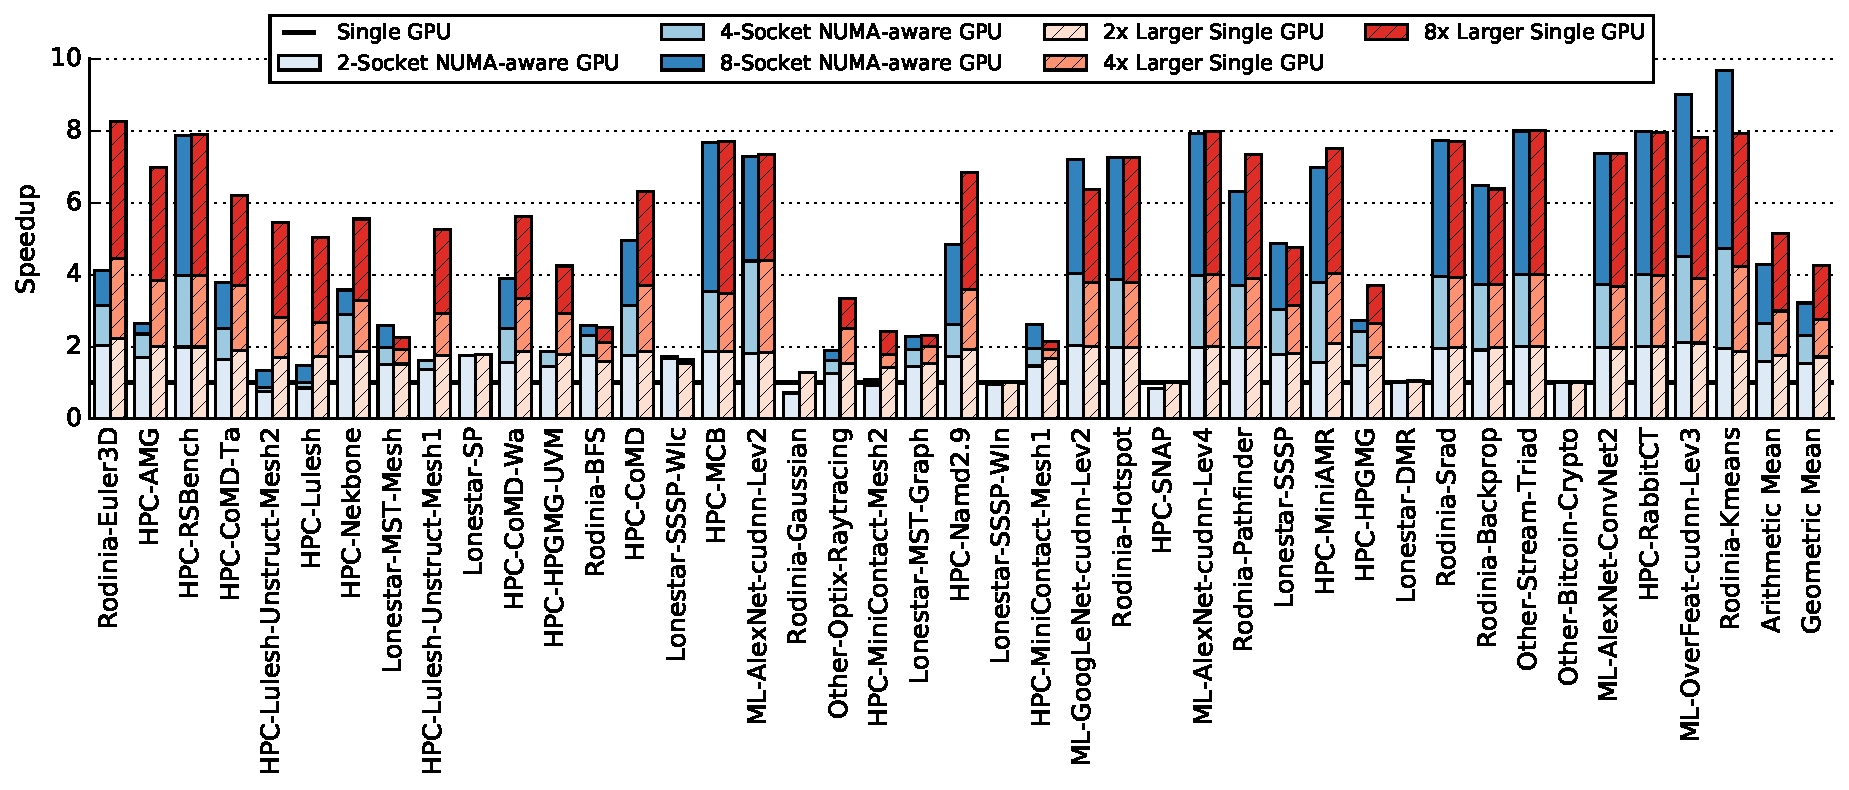
\includegraphics[width=1.0\textwidth]{figures/plot_scalability_mgpu_WB.pdf}
    \vspace{-0.05in}
    \caption{1--8 socket NUMA-aware GPU scalability compared to hypothetical larger single GPU with scaled resources.}
    \label{fig:scalability}
    \vspace{-.2in}
\end{figure*}

\vspace{-0.15in}
\section {Discussion}
\label{sec:discussion}
\textbf{Combined Improvement:} Sections~\ref{sec:interconnect} 
and~\ref{sec:caches} provide two techniques aimed at more efficiently utilizing 
scarce NUMA bandwidth within future NUMA GPU systems. The proposed methods
for dynamic interconnect balancing and NUMA-aware caching are orthogonal and 
can be applied in isolation or combination.  Dynamic interconnect balancing 
has an implementation simplicity advantage in that the system level changes to enable 
this feature are isolated from the larger GPU design.  Conversely, enabling 
NUMA-aware GPU caching based on interconnect utilization requires changes to both 
the physical cache architecture and the GPU coherence protocol.

Because these two features target the same problem, when employed 
together their effects are not strictly additive. Figure~\ref{fig:combined} 
shows the overall improvement NUMA-aware GPUs can achieve when applying 
both techniques in parallel.  For benchmarks such as \texttt{CoMD}, these 
features contribute nearly equally to the overall improvement, but for others 
such as \texttt{ML-AlexNet-cudnn-Lev2} or \texttt{HPC-MST-Mesh1}, 
interconnect improvements or caching are the primary contributor 
respectively.  On average, we observe that when combined we see 2.1$\times$ 
improvement over a single GPU and 80\% 
over the baseline software locality optimized 4-socket NUMA GPU 
using memory side L2 caches;  best performance is clearly obtained when
applying both features in unison.

\textbf{Scalability:} Ultimately, for vendors to produce multi-socket NUMA 
GPUs they must achieve high enough parallel efficiency to justify their design.  To 
understand the scalability of our approach Figure~\ref{fig:scalability} 
shows the performance of a NUMA-aware multi-socket GPU compared to a single 
GPU, when scaled across 2, 4, and 8 sockets respectively.  On average a 2 
socket NUMA GPU achieves 1.5$\times$ speedup, while 4 sockets and 8 sockets achieve 
2.3$\times$ and 3.2$\times$ speedups respectively.  Depending on perspective 
these 
speedups may look attractive or lackluster; particularly when per-benchmark 
variance is included.  However, the scalability of NUMA GPUs is not solely 
dependent on just NUMA GPU microarchitecture. We observe that for some 
applications, even if the application was run on larger hypothetical 
single GPUs, performance would scale similarly.  This may be due to a variety of 
reasons beyond NUMA effects, including number of CTAs available, frequency of 
global synchronization, and other factors.  Comparing our NUMA-aware GPU 
implementation to the scaling that applications could achieve on a hypothetical
large single GPU, we see that NUMA-GPUs can achieve 89\%, 84\%, and 76\% the
efficiency of a hypothetical single large GPU in 2, 4, and 8 socket configurations respectively.  
This high efficiency factor indicates that our design is able to largely eliminate
the NUMA penalty in future multi-socket GPU designs.

\textbf{Multi-Tenancy on Large GPUs:} In this work we have shown that many 
workloads today have the ability to saturate (with sufficient parallel work) 
a GPU that is at least 8$\times$ larger than today's GPUs.  With deep-data 
becoming commonplace across many computing paradigms, we believe that the 
trend of having enough parallel thread blocks to saturate large single GPUs will 
continue into the foreseeable future. However when GPUs become larger at the 
expense of having multiple addressable GPUs within the system, questions related 
to GPU provisioning arise.  Applications that cannot saturate large GPUs will 
leave resources underutilized and concurrently will have to multiplex across
the GPU cooperatively in time, both undesirable outcomes.

While not the focus of this work, there is significant effort in both 
industry and academia to support finer grain sharing of GPUs through either 
shared SM execution~\cite{tanasic2014enabling}, spatial multiplexing of a 
GPU~\cite{park2015chimera}, or through improved time division multiplexing 
with GPU pre-emptability~\cite{lin2016enabling}.  To support large GPU 
utilization any of these solutions could be applied to a multi-socket GPU in 
the cases where applications may not completely fill a larger GPU.  
Alternatively, with additional GPU runtime work multi-socket GPU 
designs could also be dynamically partitioned with a granularity of 
1--N logical GPUs being exposed to the programmer, providing yet another level 
of flexibility to improve utilization.

\textbf{Power Implications:} As discussed earlier, arbitrarily large monolithic 
single GPUs are unfeasible, so multi-GPU systems connected by 
high-speed links and switches may become attractive solutions for continuing 
GPU performance scaling. However, onboard high-speed links and switches 
require additional power. We estimated the link overhead by assuming $10 pJ/b$ of 
on board interconnect energy for combined links and switch (extrapolated from 
publicly available information for cabinet level Mellanox switches and 
links~\cite{mlswitch,mlnic}). Using this estimate we calculate an average 
(Geo-Mean) $30 W$ of communication power for the baseline 
architecture composed of 4 GPUs, and $14 W$ after 
our NUMA-aware optimizations are applied. Some applications such as 
\texttt{Rodinia-Euler3D, HPC-Lulesh, HPC-AMG, HPC-Lulesh-Unstruct-Mesh2} are 
communication intensive, resulting in $\approx 130 W$ of power consumption after our 
optimizations are considered. Assuming a typical TDP of $250 W$ per GPU module, 
in a 4 GPUs system, the extra power due to the communication represents a $5\%$ 
overhead across the full range of 41 evaluated benchmarks.  While this power
tax is not trivial, without alternative methods for building scalable large
GPUs, interconnect power will likely become a large portion of the overall
GPU power budget.
